% !TEX program = xelatex
\documentclass[aspectratio=169,10pt]{beamer}

% =========================
% Packages
% =========================
\usepackage{fontspec}
\usepackage{graphicx}
\usepackage{tikz}
\usetikzlibrary{calc, arrows.meta}
\usepackage{xcolor}
\usepackage{array}
\usepackage{tabularx}
\usepackage{booktabs}
\usepackage{amsmath}
\usepackage{multicol}
\usepackage{ragged2e}
\usepackage{hyperref}
\hypersetup{
  pdftitle={0.618 - Personalized Intervention Design},
  pdfauthor={Vamsi Madhav Tata},
  pdfpagemode=FullScreen
}
\usepackage{etoolbox}

% =========================
% Fonts
% =========================
\defaultfontfeatures{Ligatures=TeX}
\setmainfont{TeX Gyre Heros}
\setsansfont{TeX Gyre Heros}
\setmonofont{Latin Modern Mono}

% =========================
% Theme
% =========================
\usetheme{default}
\useinnertheme{rounded}
\useoutertheme{default}
\setbeamertemplate{navigation symbols}{}

% =========================
% Colors
% =========================
\definecolor{bg}{HTML}{F5F3EF}
\definecolor{text}{HTML}{111111}
\definecolor{muted}{HTML}{666666}
\definecolor{accent}{HTML}{6F5BFF}
\definecolor{accent2}{HTML}{3CC7B2}
\definecolor{accent3}{HTML}{FF7A59}
\definecolor{linec}{HTML}{202020}

\setbeamercolor{background canvas}{bg=bg}
\setbeamercolor{normal text}{fg=text,bg=bg}
\setbeamercolor{frametitle}{fg=text,bg=bg}
\setbeamercolor{title}{fg=text}
\setbeamercolor{subtitle}{fg=muted}
\setbeamercolor{structure}{fg=accent}
\setbeamercolor{block title}{fg=text,bg=bg}
\setbeamercolor{block body}{fg=text,bg=bg}

\setbeamerfont{title}{size=\fontsize{24}{28}\selectfont,series=\bfseries}
\setbeamerfont{subtitle}{size=\fontsize{11}{14}\selectfont}
\setbeamerfont{frametitle}{size=\fontsize{20}{22}\selectfont,series=\bfseries}
\setbeamerfont{normal text}{size=\fontsize{10.5}{13}\selectfont}

\setlength{\parskip}{0.4em}

% =========================
% Normal slide border
% =========================
\setbeamertemplate{background}{
    \begin{tikzpicture}[remember picture,overlay]
        \draw[line width=0.8pt,color=linec!35]
        ([xshift=0.5cm,yshift=0.58cm]current page.south west) rectangle
        ([xshift=-0.5cm,yshift=-0.58cm]current page.north east);
    \end{tikzpicture}
}

% =========================
% Normal slide footer
% No horizontal line
% =========================
\setbeamertemplate{footline}{
    \begin{tikzpicture}[remember picture,overlay]
        \node[anchor=south west,font=\fontsize{7}{8}\selectfont,color=muted]
        at ([xshift=0.8cm,yshift=0.09cm]current page.south west)
        {Validated Delivery 2026 - Vamsi Madhav Tata - 10046192};

        \node[anchor=south east,font=\fontsize{7}{8}\selectfont,color=muted]
        at ([xshift=-0.8cm,yshift=0.09cm]current page.south east)
        {\insertframenumber};
    \end{tikzpicture}
}

\setbeamertemplate{frametitle}{
    \vspace{0.35cm}
    \hspace{0.55cm}
    \parbox{\dimexpr\paperwidth-1.1cm\relax}{
        \raggedright\insertframetitle
    }
    \vspace{0.15cm}
}

% =========================
% Helpers
% =========================
\newcommand{\sectiontag}[1]{%
    \begin{tikzpicture}[baseline=(n.base)]
        \node[fill=accent!12,rounded corners=3pt,inner xsep=6pt,inner ysep=3pt] (n)
        {\fontsize{8}{9}\selectfont\textcolor{accent}{\textbf{#1}}};
    \end{tikzpicture}
}

\newcommand{\muted}[1]{\textcolor{muted}{#1}}
\newcommand{\accenttext}[1]{\textcolor{accent}{#1}}

\newcommand{\safeincludegraphics}[2][]{%
    \IfFileExists{#2}
        {\includegraphics[#1]{#2}}
        {%
            \begin{tikzpicture}
                \node[
                    draw=linec!40,
                    fill=black!5,
                    minimum width=6cm,
                    minimum height=4cm,
                    align=center,
                    text=muted
                ] {Missing image\\\texttt{#2}};
            \end{tikzpicture}
        }%
}

% =========================
% Full background frame
% white border + white footer
% =========================
\newcommand{\fullbgframe}[3]{%
{
\begin{frame}[plain]
\begin{tikzpicture}[remember picture,overlay]
    \IfFileExists{#1}{
        \node at (current page.center) {
            \includegraphics[width=\paperwidth]{#1}
        };
    }{
        \fill[accent!20] (current page.south west) rectangle (current page.north east);
        \node[color=white!80] at (current page.center) {\Huge Missing background image};
    }

    \fill[black,opacity=0.45] (current page.south west) rectangle (current page.north east);
    \fill[bg,opacity=0.10] (current page.south west) rectangle ([xshift=0.34\paperwidth]current page.north west);

    % White border
    \draw[line width=0.9pt,color=white!85]
    ([xshift=0.5cm,yshift=0.58cm]current page.south west) rectangle
    ([xshift=-0.5cm,yshift=-0.58cm]current page.north east);

    % White footer text
    \node[anchor=south west,font=\fontsize{7}{8}\selectfont,color=white!90]
    at ([xshift=0.8cm,yshift=0.09cm]current page.south west)
    {Validated Delivery 2026 - Vamsi Madhav Tata - 10046192};

    \node[anchor=south east,font=\fontsize{7}{8}\selectfont,color=white!90]
    at ([xshift=-0.8cm,yshift=0.09cm]current page.south east)
    {\insertframenumber};
\end{tikzpicture}

\vspace*{2.2cm}
\hspace*{1.1cm}
\begin{minipage}{0.62\paperwidth}
    {\color{white}\fontsize{30}{34}\selectfont\bfseries #2\par}
    \vspace{0.35cm}
    {\color{white!85}\fontsize{12}{16}\selectfont #3\par}
\end{minipage}
\end{frame}
}
}

% =========================
% Section Change frame
% =========================
\newcommand{\questionbgframe}[3]{%
{
\begin{frame}[plain]
\begin{tikzpicture}[remember picture,overlay]
    \IfFileExists{#1}{
        \node at (current page.center) {
            \includegraphics[width=\paperwidth]{#1}
        };
    }{
        \fill[accent!20] (current page.south west) rectangle (current page.north east);
        \node[color=white!80] at (current page.center) {\Huge Missing background image};
    }

    \fill[black,opacity=0.50] (current page.south west) rectangle (current page.north east);

    % clean white border only
    \draw[line width=0.9pt,color=white!88]
    ([xshift=0.5cm,yshift=0.58cm]current page.south west) rectangle
    ([xshift=-0.5cm,yshift=-0.58cm]current page.north east);

    % heading aligned with body text
    \node[
        anchor=north west,
        text=white,
        font=\fontsize{20}{22}\selectfont\bfseries,
        align=left
    ] at ([xshift=0.95cm,yshift=-0.65cm]current page.north west) {#2};

    % footer
    \node[anchor=south west,font=\fontsize{7}{8}\selectfont,color=white!90]
    at ([xshift=0.8cm,yshift=0.09cm]current page.south west)
    {Validated Delivery 2026 - Vamsi Madhav Tata - 10046192};

    \node[anchor=south east,font=\fontsize{7}{8}\selectfont,color=white!90]
    at ([xshift=-0.8cm,yshift=0.09cm]current page.south east)
    {\insertframenumber};
\end{tikzpicture}

\vspace*{2.25cm}
\hspace*{0.95cm}
\begin{minipage}{0.78\paperwidth}
    {\color{white}\fontsize{19}{24}\selectfont\bfseries #3\par}
\end{minipage}
\end{frame}
}
}

% =========================
% Interaction frame
% white border + white footer
% =========================
\newcommand{\interactionframe}[4]{%
{
\begin{frame}[plain]
\begin{tikzpicture}[remember picture,overlay]
    \IfFileExists{#1}{
        \node at (current page.center) {
            \includegraphics[width=\paperwidth]{#1}
        };
    }{
        \fill[accent!15] (current page.south west) rectangle (current page.north east);
        \node[color=text!70] at (current page.center) {\Huge Missing interaction image};
    }

    \fill[bg,opacity=0.80] (current page.south west) rectangle ([xshift=0.44\paperwidth]current page.north west);
    \fill[black,opacity=0.18] ([xshift=0.44\paperwidth]current page.south west) rectangle (current page.north east);

    % White border
    \draw[line width=0.9pt,color=white!85]
    ([xshift=0.5cm,yshift=0.58cm]current page.south west) rectangle
    ([xshift=-0.5cm,yshift=-0.58cm]current page.north east);

    % White footer text
    \node[anchor=south west,font=\fontsize{7}{8}\selectfont,color=white!90]
    at ([xshift=0.8cm,yshift=0.09cm]current page.south west)
    {Validated Delivery 2026 - Vamsi Madhav Tata - 10046192};

    \node[anchor=south east,font=\fontsize{7}{8}\selectfont,color=white!90]
    at ([xshift=-0.8cm,yshift=0.09cm]current page.south east)
    {\insertframenumber};
\end{tikzpicture}

\vspace*{1.55cm}
\hspace*{1.0cm}
\begin{minipage}{0.36\paperwidth}
    {\sectiontag{INTERVENTION}}
    \vspace{0.45cm}

    {\fontsize{22}{24}\selectfont\bfseries #2\par}
    \vspace{0.35cm}
    {\fontsize{10.5}{13}\selectfont #3\par}
    \vspace{0.35cm}
    {\fontsize{9}{11}\selectfont\muted{#4}\par}
\end{minipage}
\end{frame}
}
}

% =========================
% Metadata
% =========================
\title{0.618}
\subtitle{Validated Delivery 2026}
\author{Vamsi Madhav Tata}
\date{17 June 2026}

\begin{document}

% ---------------------------------
\fullbgframe{images/cover_bg.jpg}
{0.618 - Immediate and Actionable}
{A tool that helps people identify their ADHD patterns and Design their own interventions.}

% ---------------------------------
\begin{frame}{Brief Summary}
\hspace{0.7cm}
\begin{minipage}{0.84\textwidth}
{\fontsize{18}{24}\itshape
0.618 is a \accenttext{biofeedback based tool} that people with ADHD can use to build their own personalized interventions, \accenttext{through instant feedback.}}
\end{minipage}

\vspace{0.8cm}

\hspace{0.7cm}
\begin{minipage}{0.84\textwidth}
\muted{The project is not proposing one universal intervention. It is proposing a prototype tool through which interventions can be explored, compared, and personalised.}
\end{minipage}
\end{frame}

% ---------------------------------
\begin{frame}{Project Overview}
\begin{tikzpicture}[remember picture,overlay]

% =========================================================
% LAYOUT AREA
% =========================================================
\coordinate (A) at ([xshift=1.10cm,yshift=-1.70cm]current page.north west);
\coordinate (B) at ([xshift=-1.10cm,yshift=1.55cm]current page.south east);

% ---------------------------------------------------------
% LEFT : circular tool/platform
% ---------------------------------------------------------
\node[anchor=north west,text=text]
at ([xshift=0.05cm,yshift=0cm]A)
{\fontsize{13}{15}\selectfont\bfseries Tool / Platform};

\coordinate (L) at ([xshift=2.05cm,yshift=-2.55cm]A);

% circular image crop
\begin{scope}
    \clip (L) circle (1.55cm);
    \IfFileExists{images/tool_platform.jpg}{
        \node at (L) {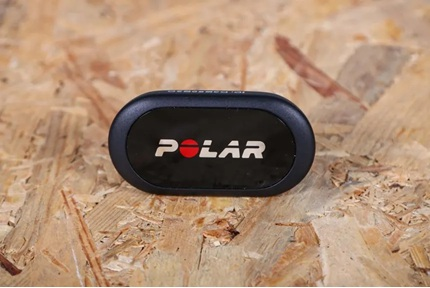
\includegraphics[scale=0.5]{images/tool_platform.jpg}};
    }{
        \fill[black!5] (L) circle (1.55cm);
        \node[text=muted,align=center] at (L) {\fontsize{10}{12}\selectfont tool\\image};
    }
\end{scope}
\draw[line width=0.9pt,color=linec!60] (L) circle (1.55cm);

\node[anchor=north west,text=text]
at ([xshift=0.25cm,yshift=-5.15cm]A)
{\fontsize{10.5}{12.5}\selectfont\bfseries Sensor};

\node[anchor=north west,text=muted,align=left, text width = 4.5cm]
at ([xshift=0.25cm,yshift=-5.60cm]A)
{\fontsize{8.8}{10.6}\selectfont
Tracks Heart rate, Heart rate variance, and Breathing rate};

% ---------------------------------------------------------
% MIDDLE : current output
% ---------------------------------------------------------
\node[anchor=north west,text=text]
at ([xshift=4.95cm,yshift=0cm]A)
{\fontsize{13}{15}\selectfont\bfseries Current Output};

\coordinate (M1) at ([xshift=5.05cm,yshift=-1.15cm]A);
\coordinate (M2) at ([xshift=9.05cm,yshift=-4.35cm]A);

% rounded rectangle image crop
\begin{scope}
    \clip[rounded corners=16pt] (M1) rectangle (M2);
    \IfFileExists{images/current_output.jpeg}{
        \node at ($(M1)!0.5!(M2)$)
        {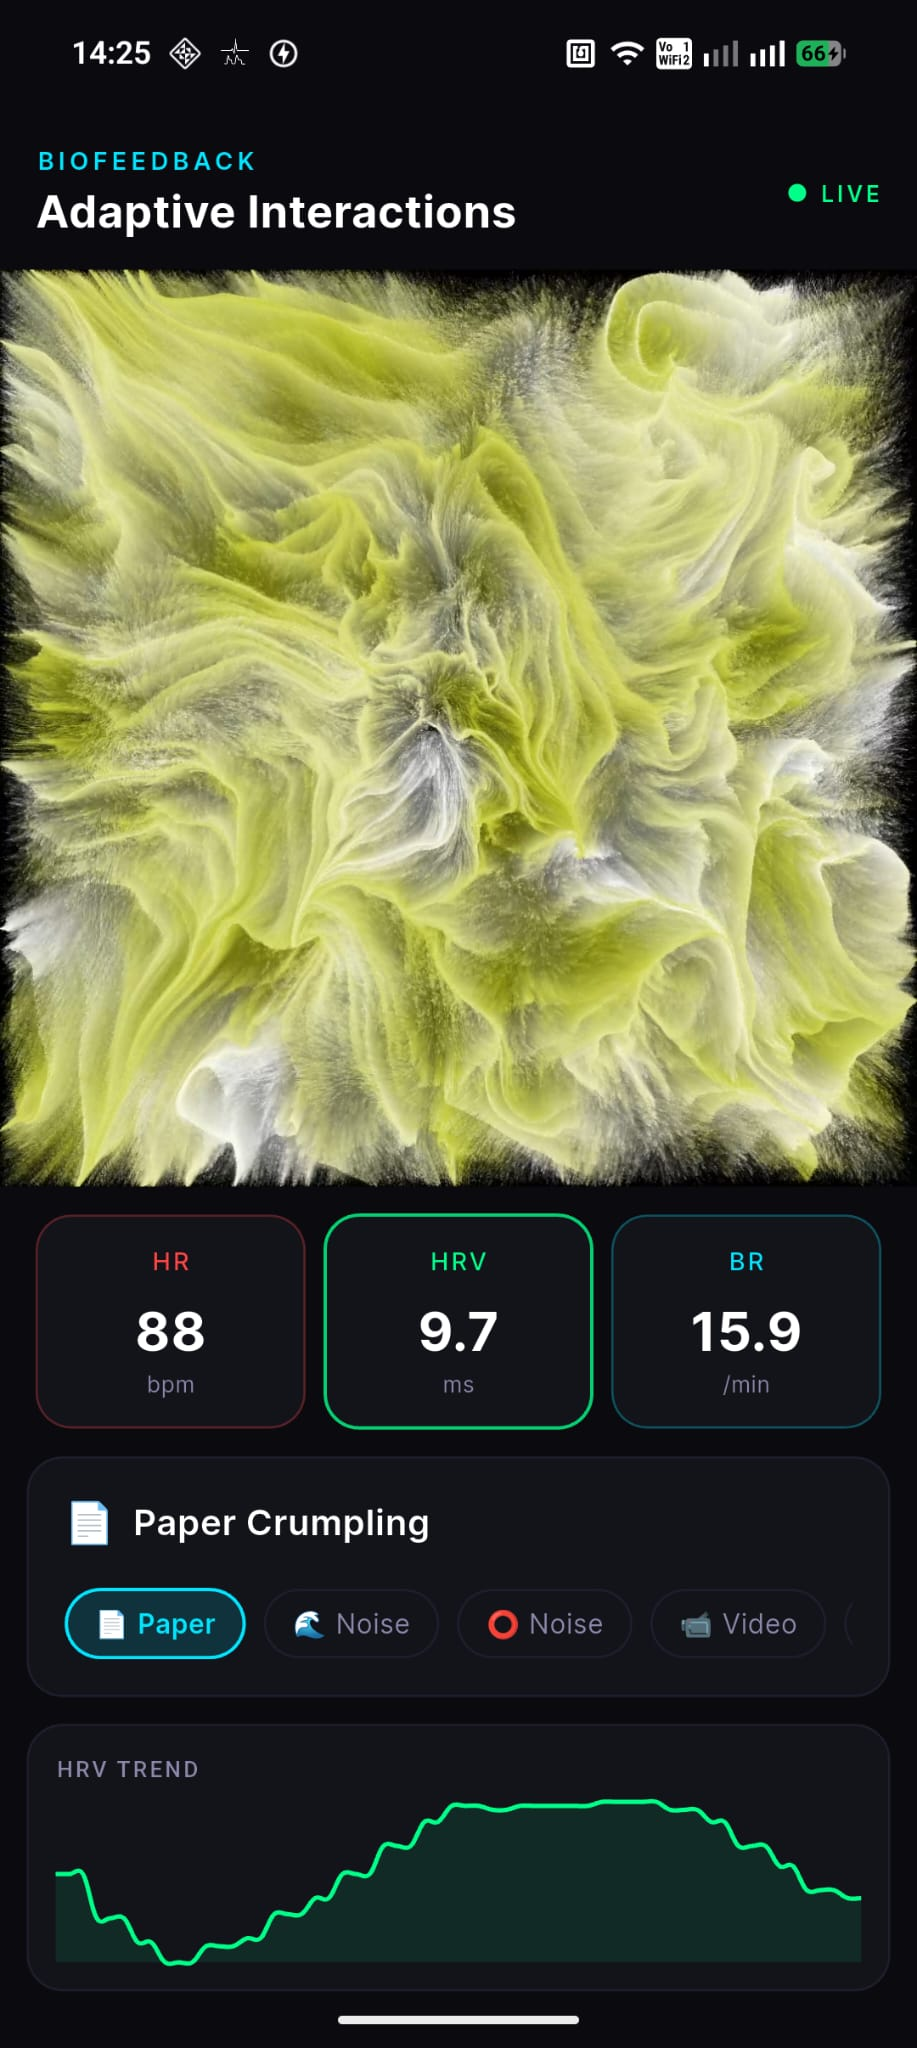
\includegraphics[scale = 0.125]{images/current_output.jpeg}};
    }{
        \fill[black!5,rounded corners=16pt] (M1) rectangle (M2);
        \node[text=muted,align=center] at ($(M1)!0.5!(M2)$)
        {\fontsize{10}{12}\selectfont current\\output};
    }
\end{scope}
\draw[line width=0.9pt,color=linec!60,rounded corners=16pt] (M1) rectangle (M2);

\node[anchor=north west,text=text]
at ([xshift=5.05cm,yshift=-5.15cm]A)
{\fontsize{10.5}{12.5}\selectfont\bfseries Interaction output};

\node[anchor=north west,text=muted,align=left, text width = 4.5 cm]
at ([xshift=5.05cm,yshift=-5.60cm]A)
{\fontsize{8.8}{10.6}\selectfont
App streaming the TD output operated by RL model};

\draw[dashed, thick] ([xshift = 9.75 cm]A) -- ([xshift = 9.75 cm, yshift = -6.5 cm]A);

% ---------------------------------------------------------
% RIGHT : intervention set
% ---------------------------------------------------------
\node[anchor=north west,text=text]
at ([xshift=10.30cm,yshift=0cm]A)
{\fontsize{13}{15}\selectfont\bfseries Intervention Set};

\coordinate (R1) at ([xshift=10.45cm,yshift=-1.00cm]A);
\coordinate (R2) at ([xshift=14.15cm,yshift=-4.35cm]A);

% front crop
\begin{scope}
    \clip[rounded corners=16pt] (R1) rectangle (R2);
    \IfFileExists{images/intervention_set.jpg}{
        \node[xshift =-1.5cm] at ($(R1)!0.5!(R2)$)
        {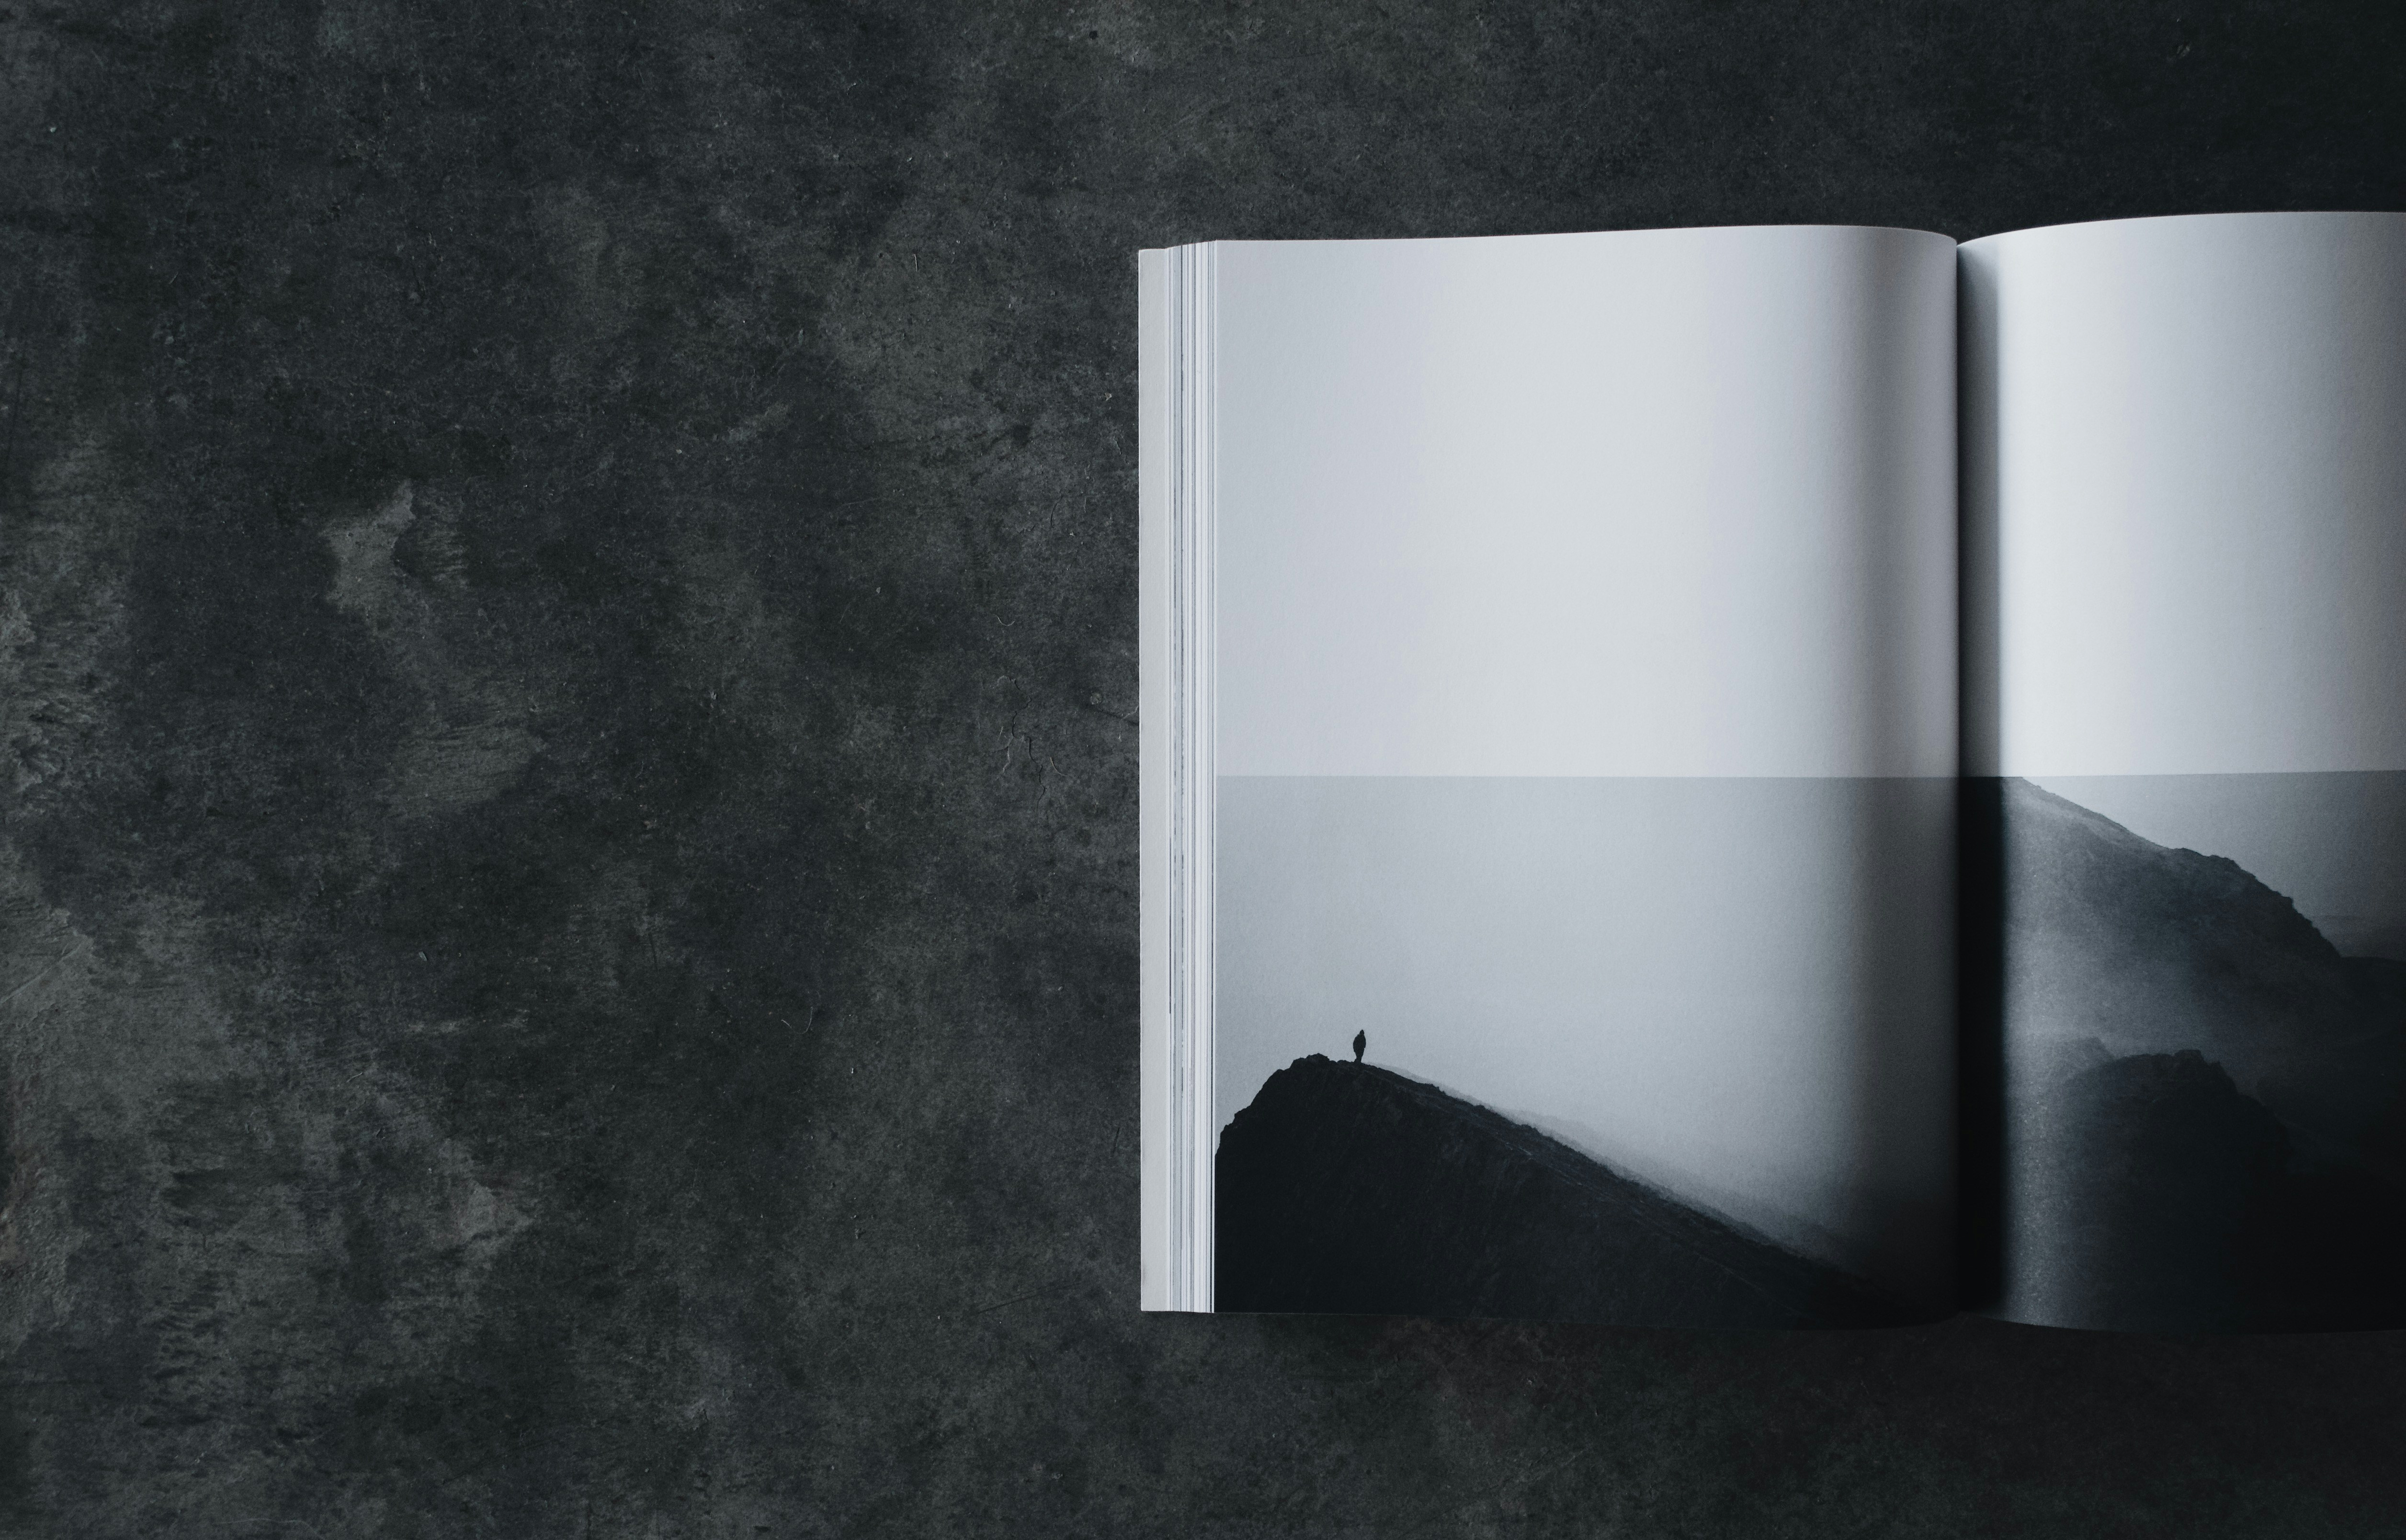
\includegraphics[scale = 0.15]{images/intervention_set.jpg}};
    }{
        \fill[black!5,rounded corners=16pt] (R1) rectangle (R2);
        \node[text=muted,align=center] at ($(R1)!0.5!(R2)$)
        {\fontsize{10}{12}\selectfont intervention\\set};
    }
\end{scope}
\draw[line width=0.9pt,color=linec!60,rounded corners=16pt] (R1) rectangle (R2);

\node[anchor=north west,text=text]
at ([xshift=10.38cm,yshift=-5.15cm]A)
{\fontsize{10.5}{12.5}\selectfont\bfseries Intervention set};

\node[anchor=north west,text=muted,align=left, text width = 3.75cm]
at ([xshift=10.38cm,yshift=-5.60cm]A)
{\fontsize{8.8}{10.6}\selectfont
Recommended by Expert to include this starter list};

\end{tikzpicture}
\end{frame}

% ---------------------------------

\begin{frame}{Why ADHD matters?}
\hspace{0.7cm}
\begin{minipage}{0.84\textwidth}
{\fontsize{18}{24}\itshape
"Research by psychologist Dr. Russell Barkley, a prominent ADHD researcher, demonstrates that ADHD has a \textcolor{red}{significantly negative impact on
life expectancy — by 12.7 years, on average.} ADHD makes our lives \accenttext{harder and shorter.}}"
\end{minipage}
\end{frame}

% ---------------------------------

\begin{frame}{Why 0.618 matters??}
\begin{tikzpicture}[remember picture,overlay, x=1cm, y=1cm]

% -----------------------------
% layout controls
% -----------------------------
\def\leftx{1.45}
\def\topY{3.5}
\def\boxW{2.3}
\def\boxH{2.3}
\def\colGap{1.00}
\def\arrowGap{0.60}
\def\bottomGap{0.62}

% column x positions
\pgfmathsetmacro{\xA}{\leftx}
\pgfmathsetmacro{\xB}{\xA + \boxW + \colGap}
\pgfmathsetmacro{\xC}{\xB + \boxW + \colGap}
\pgfmathsetmacro{\xD}{\xC + \boxW + \colGap}

% y positions
\pgfmathsetmacro{\yTop}{\topY}
\pgfmathsetmacro{\yBot}{\yTop - \boxH - \arrowGap}

% style
\tikzset{
  logicbox/.style={
    draw=linec!55,
    rounded corners=9pt,
    line width=0.85pt
  }
}

% =========================================================
% COLUMN 1
% =========================================================

% top square
\draw[logicbox] (\xA,\yTop) rectangle ++(\boxW,-\boxH);

\begin{scope}
    \clip[rounded corners=9pt] (\xA,\yTop) rectangle ++(\boxW,-\boxH);
    \fill[black!2] (\xA,\yTop) rectangle ++(\boxW,-\boxH);
    \foreach \i in {-1.0,-0.7,...,3.5}{
        \draw[line width=0.32pt,color=linec!22]
        (\xA+\i,\yTop-\boxH-0.08) -- (\xA+\i+2.3,\yTop+0.10);
    }
\end{scope}

\foreach \cx/\cy in {
0.38/0.35, 0.88/0.34, 1.38/0.34, 1.88/0.35,
0.60/0.86, 1.15/0.86, 1.65/0.86,
0.38/1.37, 0.88/1.37, 1.38/1.37, 1.88/1.37,
0.62/1.78, 1.16/1.78, 1.70/1.78}
{
    \filldraw[fill=bg,draw=linec!38,line width=0.32pt]
    (\xA+\cx,\yTop-\cy) circle (0.09);
}

\draw[->,line width=0.68pt,color=linec!55]
(\xA+1.12,\yTop-\boxH-0.12) -- (\xA+1.12,\yTop-\boxH-0.42);

% bottom square
\draw[logicbox] (\xA,\yBot) rectangle ++(\boxW,-\boxH);

\foreach \cx/\cy/\c in {
0.40/0.42/red!78, 0.90/0.45/blue!78, 1.40/0.42/green!78, 1.85/0.45/purple!78,
0.65/0.83/blue!70, 1.15/0.86/green!70, 1.65/0.83/red!70,
0.40/1.28/purple!70, 0.90/1.31/green!72, 1.40/1.28/blue!72, 1.85/1.31/red!72,
0.66/1.72/green!70, 1.18/1.74/purple!76, 1.70/1.70/blue!70}
{
    \filldraw[fill=\c,draw=linec!24,line width=0.28pt]
    (\xA+\cx,\yBot-\cy) circle (0.08);
}

\node[anchor=north west,text=muted,align=left,text width=3cm]
at (\xA,\yBot-\boxH-0.10)
{\fontsize{7.2}{8.8}\selectfont
“What works best can depend on the child and family.” - CDC};

% =========================================================
% COLUMN 2
% =========================================================

\draw[logicbox] (\xB,\yTop) rectangle ++(\boxW,-\boxH);

\begin{scope}
    \clip[rounded corners=9pt] (\xB,\yTop) rectangle ++(\boxW,-\boxH);
    \node at (\xB+0.5*\boxW,\yTop-0.5*\boxH)
    {
\includegraphics[width=\boxW cm,height=\boxH cm]{images/prescribed.jpg}};
\end{scope}

\draw[->,line width=0.68pt,color=linec!55]
(\xB+1.12,\yTop-\boxH-0.12) -- (\xB+1.12,\yTop-\boxH-0.42);

\draw[logicbox] (\xB,\yBot) rectangle ++(\boxW,-\boxH);

\begin{scope}
    \clip[rounded corners=9pt] (\xB,\yBot) rectangle ++(\boxW,-\boxH);
    \node at (\xB+0.5*\boxW,\yBot-0.5*\boxH)
    {
\includegraphics[width=\boxW cm,height=\boxH cm]{images/discovery.jpg}};
\end{scope}

\node[anchor=north west,text=muted,align=left,text width=3cm]
at (\xB,\yBot-\boxH-0.10)
{\fontsize{7}{8.8}\selectfont
"A study of 9 million GP records showed just 0.32\% had a diagnosis of ADHD."};
% =========================================================
% COLUMN 3
% =========================================================

\draw[logicbox] (\xC,\yTop) rectangle ++(\boxW,-\boxH);

\begin{scope}
    \clip[rounded corners=9pt] (\xC,\yTop) rectangle ++(\boxW,-\boxH);
    \node at (\xC+0.5*\boxW,\yTop-0.5*\boxH)
    {
\includegraphics[width=\boxW cm,height=\boxH cm]{images/retrospective.jpg}};
\end{scope}

\draw[->,line width=0.68pt,color=linec!55]
(\xC+1.12,\yTop-\boxH-0.12) -- (\xC+1.12,\yTop-\boxH-0.42);

\draw[logicbox] (\xC,\yBot) rectangle ++(\boxW,-\boxH);

\begin{scope}
    \clip[rounded corners=9pt] (\xC,\yBot) rectangle ++(\boxW,-\boxH);
    \node at (\xC+0.5*\boxW,\yBot-0.5*\boxH)
    {
\includegraphics[width=\boxW cm,height=\boxH cm]{images/inthemoment.jpg}};
\end{scope}

\node[anchor=north west,text=muted,align=left,text width=3cm]
at (\xC,\yBot-\boxH-0.10)
{\fontsize{7.2}{8.8}\selectfont
"People With ADHD lack self-awareness" - Rosemary Briggs RCA disability advisor};

% =========================================================
% COLUMN 4
% =========================================================

\draw[logicbox] (\xD,\yTop) rectangle ++(\boxW,-\boxH);

\begin{scope}
    \clip[rounded corners=9pt] (\xD,\yTop) rectangle ++(\boxW,-\boxH);
    \node at (\xD+0.5*\boxW,\yTop-0.5*\boxH)
    {
\includegraphics[width=\boxW cm,height=\boxH cm]{images/ramp.jpg}};
\end{scope}

\draw[->,line width=0.68pt,color=linec!55]
(\xD+1.12,\yTop-\boxH-0.12) -- (\xD+1.12,\yTop-\boxH-0.42);

\draw[logicbox] (\xD,\yBot) rectangle ++(\boxW,-\boxH);

\begin{scope}
    \clip[rounded corners=9pt] (\xD,\yBot) rectangle ++(\boxW,-\boxH);
    \node at (\xD+0.5*\boxW,\yBot-0.5*\boxH)
    {
\includegraphics[width=\boxW cm,height=\boxH cm]{images/3mins.jpg}};
\end{scope}

\node[anchor=north west,text=muted,align=left,text width=3cm]
at (\xD,\yBot-\boxH-0.10)
{\fontsize{7.2}{8.8}\selectfont
"I built up this toolbox over seven years, learning one tool a week... Jessica McCabe”};

\end{tikzpicture}
\end{frame}

% ---------------------------------

\begin{frame}{Context Validation}
\hspace{0.7cm}
\begin{minipage}{0.84\textwidth}
{\fontsize{18}{24}\itshape
"\textcolor{red}{I was constantly angry when I was taking my medication" - (Anonymous)} \vspace{0.5cm} \\  \textcolor{accent}{"As someone from a family with ADHD, I saw my sister get significantly less creative because of meds. As a design professional, I can not afford that" - (Anonymous)}}
\end{minipage}
\end{frame}

% ---------------------------------
\questionbgframe
{images/do.jpg}
{The Design Opportunity}
{How might we help people with ADHD identify their \textcolor{yellow}{patterns at the moment} and build personalized, actionable interventions \textcolor{yellow}{through immediate feedback?}}

%----------------------------------

\begin{frame}{Demo}
\hspace{0.7cm}
\begin{minipage}{0.84\textwidth}
{\fontsize{36}{42}\selectfont\bfseries
\hspace{4cm} Demo}
\end{minipage}
\end{frame}

% ---------------------------------
\begin{frame}{Current Prototype Outcome}
\begin{tikzpicture}[remember picture,overlay, x=1cm, y=1cm]

% ---------------------------------------------------------
% layout anchor
% ---------------------------------------------------------
\coordinate (A) at ([xshift=1.05cm,yshift=-1.70cm]current page.north west);

% sizes tuned to fit inside existing frame + footer
\def\imgW{4.20}
\def\imgH{6.45}
\def\midW{3.35}
\def\midH{3.75}

% x positions
\def\xL{1.00}
\def\xM{6.00}
\def\xR{10.00}

% y positions
\def\yTop{0.15}

% =========================================================
% LEFT IMAGE
% =========================================================
\coordinate (L1) at ([xshift=\xL cm,yshift=-\yTop cm]A);
\coordinate (L2) at ([xshift=\xL cm+\imgW cm,yshift=-\yTop cm-\imgH cm]A);

\begin{scope}
    \clip[rounded corners=16pt] (L1) rectangle (L2);
    \node at ($(L1)!0.5!(L2)$)
    {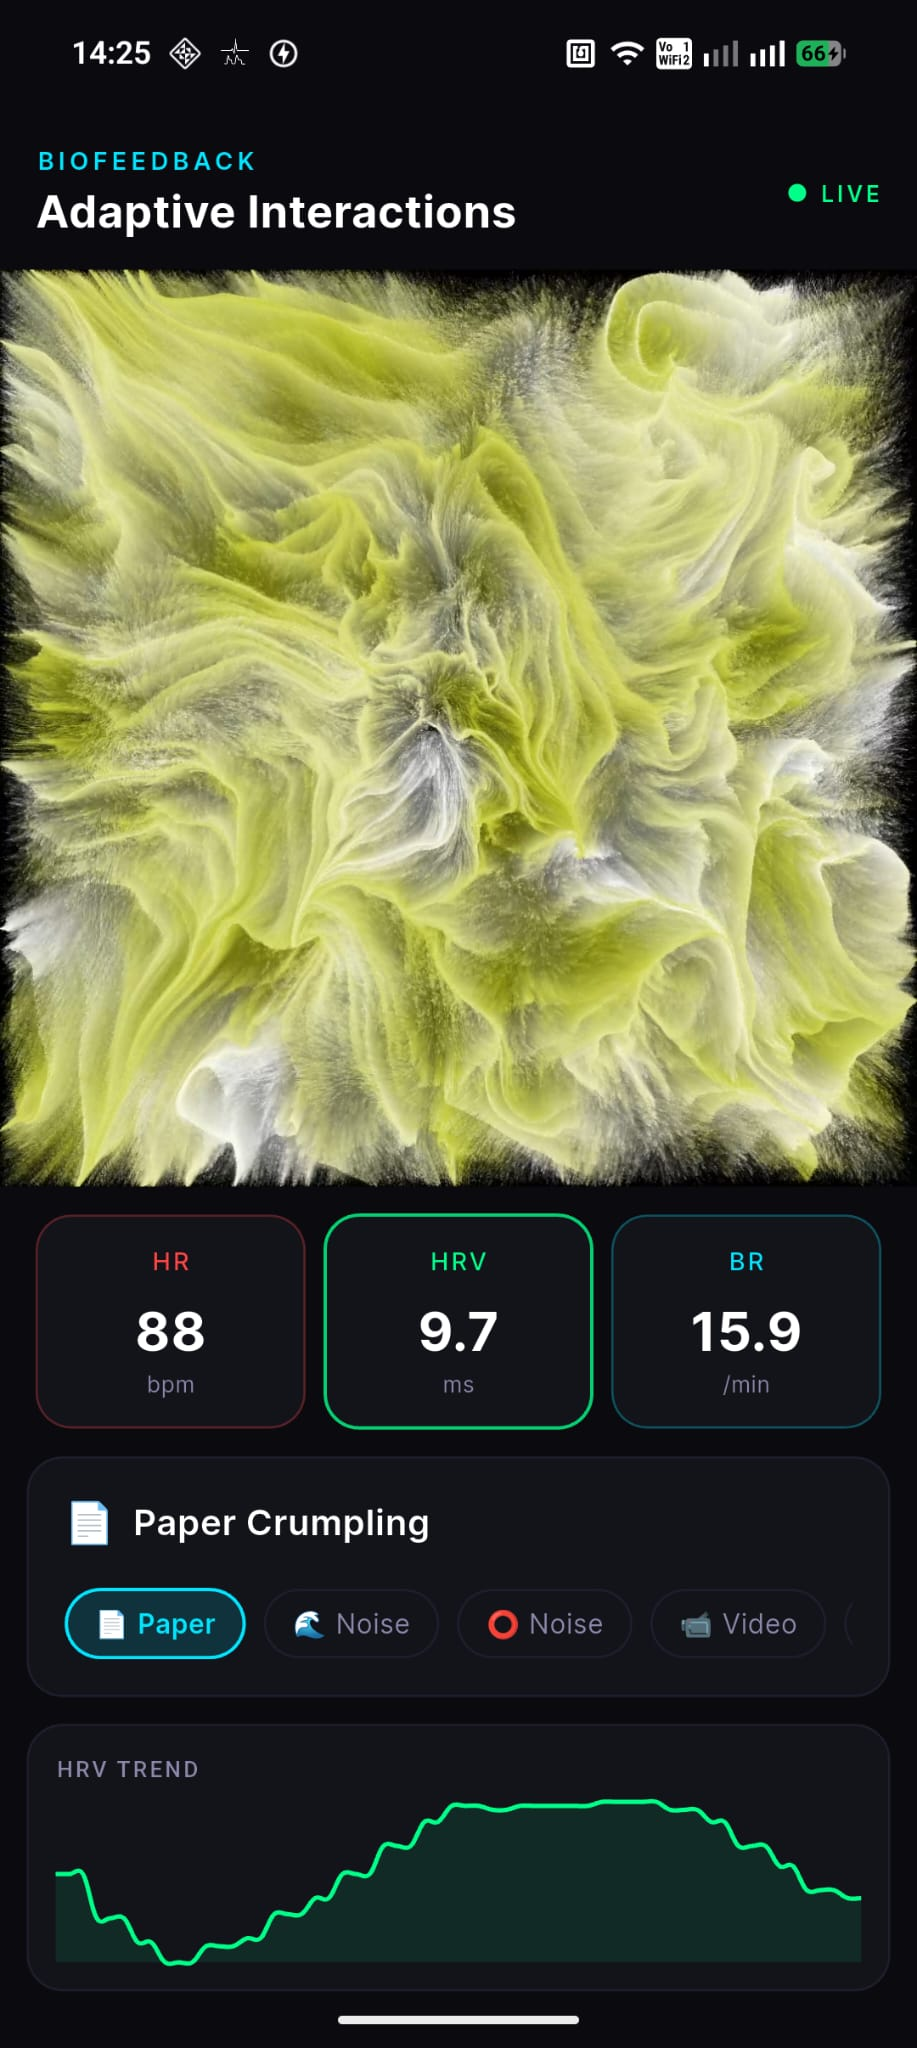
\includegraphics[scale=0.15]{images/current_output.jpeg}};
\end{scope}
\draw[line width=0.9pt,color=linec!58,rounded corners=16pt] (L1) rectangle (L2);

% =========================================================
% CENTER : JULIA + TOUCHDESIGNER
% =========================================================
\coordinate (M1) at ([xshift=\xM cm,yshift=-0.95cm]A);
\coordinate (M2) at ([xshift=\xM cm+\midW cm,yshift=-0.95cm-\midH cm]A);

\draw[line width=0.85pt,color=linec!42,dashed,rounded corners=10pt]
(M1) rectangle (M2);

\node[text=text] at ($(M1)!0.5!(M2)+(0,0.85)$)
{\fontsize{15}{17}\selectfont\bfseries Julia};

\node[text=text] at ($(M1)!0.5!(M2)+(0,0.25)$)
{\fontsize{16}{18}\selectfont +};

\node[text=text,align=center] at ($(M1)!0.5!(M2)+(-0.10,-0.65)$)
{\fontsize{14}{16}\selectfont Touch\\Designer};

% =========================================================
% RIGHT IMAGE
% =========================================================
\coordinate (R1) at ([xshift=\xR cm,yshift=-\yTop cm]A);
\coordinate (R2) at ([xshift=\xR cm+\imgW cm,yshift=-\yTop cm-\imgH cm]A);

\begin{scope}
    \clip[rounded corners=16pt] (R1) rectangle (R2);
    \node at ($(R1)!0.5!(R2)$)
    {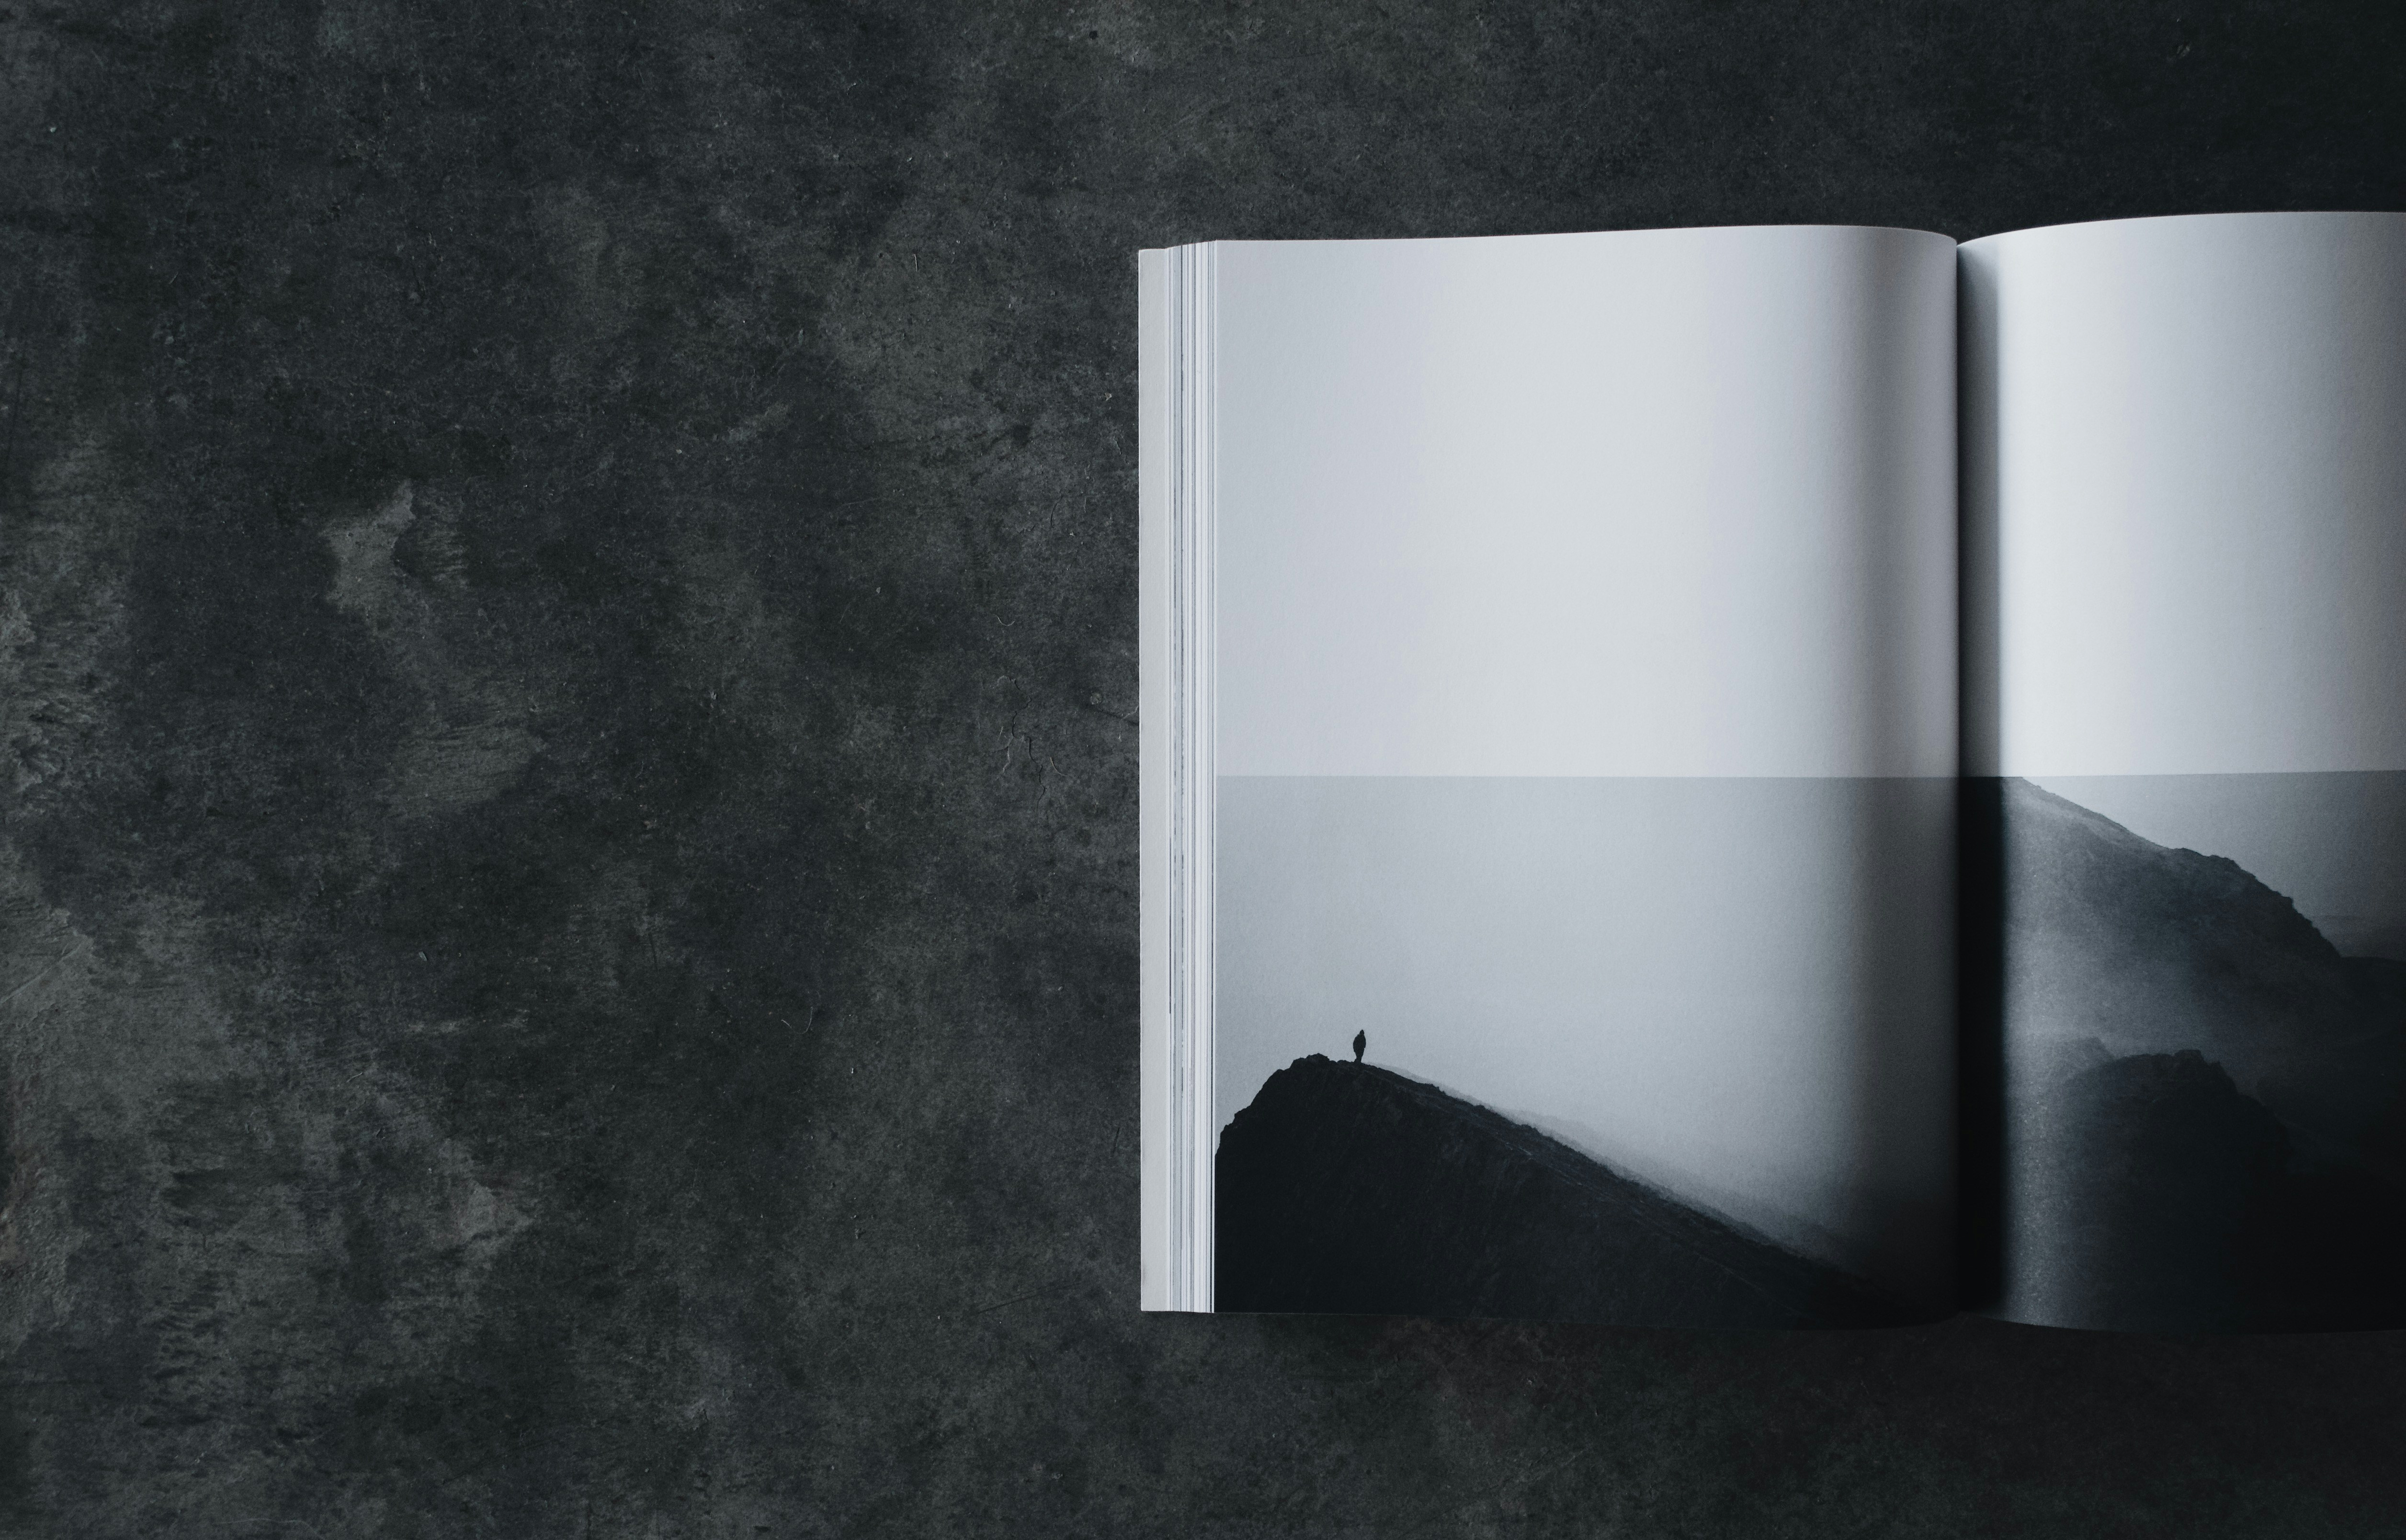
\includegraphics[scale=0.2]{images/intervention_set.jpg}};
\end{scope}
\draw[line width=0.9pt,color=linec!58,rounded corners=16pt] (R1) rectangle (R2);

\end{tikzpicture}
\end{frame}
% ---------------------------------

\begin{frame}{System Architecture}
\begin{tikzpicture}[remember picture,overlay]

% --- rectangle coordinates
\coordinate (P1) at ([xshift=1.2cm,yshift=-1.8cm]current page.north west);
\coordinate (P2) at ([xshift=-1.2cm,yshift=1cm]current page.south east);

% --- clipped rounded rectangle image
\begin{scope}
    \clip[rounded corners=14pt] (P1) rectangle (P2);
    \node at ($(P1)!0.5!(P2)$)
    {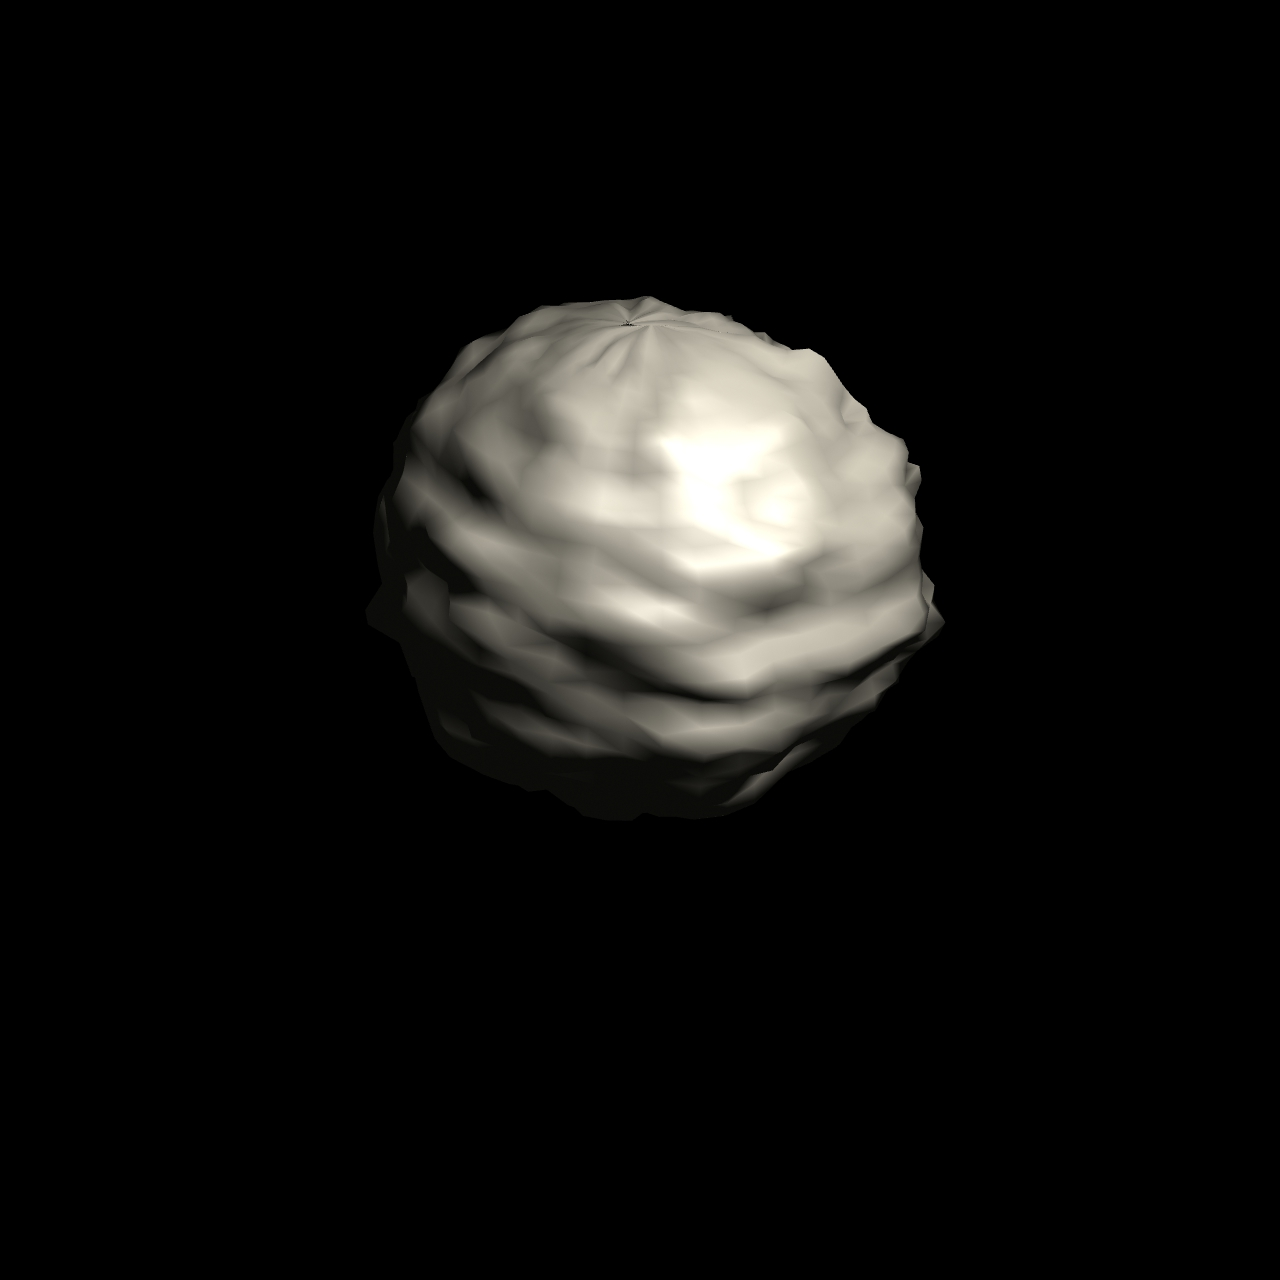
\includegraphics[width=14.5cm,height=7.4cm]{images/interaction_01.jpg}};
\end{scope}

% --- rounded rectangle border
\draw[line width=0.9pt,color=linec!60,rounded corners=14pt] (P1) rectangle (P2);

\end{tikzpicture}
\end{frame}

% ---------------------------------
\begin{frame}{What has been built}
\begin{columns}[T,totalwidth=\textwidth]
\column{0.33\textwidth}
\hspace{0.45cm}
\begin{minipage}{0.86\linewidth}
\sectiontag{APP}

\vspace{0.25cm}
\begin{itemize}
    \item live vitals display
    \item HR / HRV trend view
    \item manual triggers
    \item calendar triggers
    \item camera stream control
\end{itemize}
\end{minipage}

\column{0.33\textwidth}
\begin{minipage}{0.9\linewidth}
\sectiontag{BACKEND}

\vspace{0.25cm}
\begin{itemize}
    \item data ingestion
    \item windowing
    \item temporal encoding
    \item RL / state logic
    \item status reporting
\end{itemize}
\end{minipage}

\column{0.34\textwidth}
\begin{minipage}{0.9\linewidth}
\sectiontag{MEDIA}

\vspace{0.25cm}
\begin{itemize}
    \item interaction switching
    \item hold progress
    \item audiovisual output
    \item remote / local stream support
\end{itemize}
\end{minipage}
\end{columns}
\end{frame}

% ---------------------------------
\begin{frame}{Development through prototyping}
\hspace{0.7cm}
\begin{minipage}{0.88\textwidth}
\sectiontag{PROTOTYPING}

\vspace{0.35cm}
The project developed through several prototype layers:

\vspace{0.2cm}
\begin{tabularx}{0.9\textwidth}{>{\bfseries}p{0.22\textwidth}X}
Signal prototype & extracting and processing physiological data from the Polar H10 \\
System prototype & app, backend, and interaction pipeline working together \\
Intervention prototype & initial intervention modes available to trigger and compare \\
Interaction prototype & media outputs tested as short-form interventions \\
Wearable direction & future transition from chest strap to ring-based sensing \\
\end{tabularx}
\end{minipage}
\end{frame}

% ---------------------------------
\interactionframe
{images/interaction_01.jpg}
{Intervention 01}
{A ready-to-go intervention intended as a starting point for testing and comparison.}
{Dummy image placeholder — replace with final visual.}

\interactionframe
{images/interaction_02.jpg}
{Intervention 02}
{A contrasting mode exploring a different sensory or interaction strategy.}
{Dummy image placeholder — replace with final visual.}

\interactionframe
{images/interaction_03.jpg}
{Intervention 03 — Video Ripples}
{A more embodied intervention mode using live camera input through the app.}
{In the current system, this interaction activates local camera streaming.}

\interactionframe
{images/interaction_04.jpg}
{Intervention 04}
{Another testable intervention mode in the current set.}
{Dummy image placeholder — replace with final visual.}

\interactionframe
{images/interaction_05.jpg}
{Intervention 05}
{A fifth mode expanding the current intervention library.}
{Dummy image placeholder — replace with final visual.}

% ---------------------------------
\begin{frame}{How the interventions are being used}
\hspace{0.7cm}
\begin{minipage}{0.87\textwidth}
The current interventions are not presented as final or universal solutions.

\vspace{0.35cm}

They function as:
\begin{itemize}
    \item ready-to-go starting points
    \item testable patterns
    \item a way to compare different forms of support
    \item a basis for future personalization
\end{itemize}

\vspace{0.45cm}
\muted{The project contribution is therefore the tool + the current intervention set + the logic for testing them in short windows.}
\end{minipage}
\end{frame}

% ---------------------------------
\begin{frame}{Current validation}
\begin{columns}[T,totalwidth=\textwidth]
\column{0.52\textwidth}
\hspace{0.55cm}
\begin{minipage}{0.9\linewidth}
\sectiontag{VALIDATED SO FAR}

\vspace{0.35cm}
Current validation focuses on:
\begin{itemize}
    \item \textbf{technical feasibility} — the system operates across sensing, app, backend, and media layers
    \item \textbf{integration} — multiple components can work together end-to-end
    \item \textbf{desirability / interest} — early evidence suggests that users or stakeholders find the idea relevant and compelling
\end{itemize}
\end{minipage}

\column{0.48\textwidth}
\vspace{0.25cm}
\safeincludegraphics[width=0.92\linewidth]{images/validation.jpg}
\end{columns}
\end{frame}

% ---------------------------------
\begin{frame}{What is not yet validated}
\hspace{0.7cm}
\begin{minipage}{0.88\textwidth}
\sectiontag{NOT YET CLAIMED}

\vspace{0.35cm}
This project does \textbf{not yet claim}:
\begin{itemize}
    \item validated effectiveness for ADHD users
    \item tested personalization outcomes
    \item formal user testing across the intervention set
    \item everyday deployment through the future ring hardware
\end{itemize}

\vspace{0.45cm}
Instead, the current contribution is a \textbf{credible prototype platform} that makes those next validation stages possible.
\end{minipage}
\end{frame}

% ---------------------------------
\begin{frame}{Evidence generated, so far}
\hspace{0.7cm}
\begin{minipage}{0.88\textwidth}
Evidence produced through development includes:

\begin{itemize}
    \item a functioning app interface
    \item live status and physiological history display
    \item working trigger pathways
    \item successful intervention switching
    \item functioning camera activation for one intervention mode
    \item backend state, reward, and debug tracking
    \item early validation that the proposition is interesting and relevant to people
\end{itemize}
\end{minipage}
\end{frame}

% ---------------------------------
\begin{frame}{Current limitations}
\hspace{0.7cm}
\begin{minipage}{0.88\textwidth}
\begin{itemize}
    \item user testing is still to be completed
    \item personalization is a project direction, not yet a validated outcome
    \item the current sensing setup still relies on the Polar H10
    \item the ring has not yet been built
    \item intervention effectiveness has not yet been comparatively evaluated with users
\end{itemize}

\vspace{0.45cm}
\textbf{This is important:} the project is presented here as a technically resolved prototype and a clear next-stage proposition, not as a finished validated product.
\end{minipage}
\end{frame}

% ---------------------------------
\begin{frame}{Future scope}
\begin{columns}[T,totalwidth=\textwidth]
\column{0.52\textwidth}
\hspace{0.55cm}
\begin{minipage}{0.9\linewidth}
\sectiontag{NEXT STEPS}

\vspace{0.35cm}
Next phases include:
\begin{itemize}
    \item user testing with ADHD participants
    \item comparative testing across interventions
    \item evaluating whether short-window use is meaningful
    \item refining how users identify useful strategies
\end{itemize}
\end{minipage}

\column{0.48\textwidth}
\begin{minipage}{0.88\linewidth}
\sectiontag{HARDWARE DIRECTION}

\vspace{0.35cm}
Future hardware development includes:
\begin{itemize}
    \item replacing the Polar H10 with a ring
    \item improving comfort and every day use
    \item reducing friction in real-world use
    \item moving from prototype sensing toward embedded support
\end{itemize}
\end{minipage}
\end{columns}
\end{frame}

% ---------------------------------
\begin{frame}{Conclusion}
\hspace{0.7cm}
\begin{minipage}{0.85\textwidth}
{\fontsize{18}{24}\selectfont\bfseries
This project does not present a single fixed intervention. It presents a prototype system through which personalised ADHD interventions could be explored, tested, and developed over time.}

\vspace{0.6cm}

It currently demonstrates:
\begin{itemize}
    \item a working technical prototype
    \item an initial intervention set
    \item integration of design and engineering
    \item early evidence of interest and relevance
    \item a clear path toward future user testing and wearable refinement
\end{itemize}
\end{minipage}
\end{frame}

% ---------------------------------
\begin{frame}{Statement of originality}
\hspace{0.7cm}
\begin{minipage}{0.88\textwidth}
\small
This project is my own original work. All external sources, references, images, code libraries, and ideas have been clearly acknowledged within the presentation or supporting material. Except where indicated, all other material presented here is my own.

\vspace{0.55cm}

\textbf{Acknowledgements}
\begin{itemize}
    \item Flutter, Julia, and supporting package ecosystems
    \item Google Calendar, WebRTC, and other third-party libraries where used
    \item Touch Designer integration and any external technical or conceptual advice to be credited here as appropriate
\end{itemize}
\end{minipage}
\end{frame}

% ---------------------------------
\fullbgframe{images/cover_bg.jpg}
{Thank you}
{Questions}

% ---------------------------------

\begin{frame}{Why the 3-minute window matters}
\begin{columns}[T,totalwidth=\textwidth]
\column{0.54\textwidth}
\hspace{0.55cm}
\begin{minipage}{0.9\linewidth}
\sectiontag{BEHAVIOURAL WINDOW}

\vspace{0.35cm}
The intervention window is intentionally short.

\vspace{0.25cm}
This matters because:
\begin{itemize}
    \item ADHD-related behaviour can shift rapidly
    \item support is often needed in the moment, not after the fact
    \item shorter windows make experimentation more repeatable
    \item brief trials allow users to compare responses and preferences
\end{itemize}
\end{minipage}

\column{0.46\textwidth}
\hspace{0.0cm}
\begin{minipage}{0.88\linewidth}
\sectiontag{PROJECT AIM}

\vspace{0.35cm}
The goal is not to ``fix'' attention in three minutes.

The goal is to create a structure in which users can:
\begin{itemize}
    \item notice a shift
    \item engage a candidate intervention
    \item observe what helps
    \item build personal insight over time
\end{itemize}
\end{minipage}
\end{columns}
\end{frame}

% ---------------------------------
\begin{frame}{Design and engineering challenge}
\begin{columns}[T,totalwidth=\textwidth]
\column{0.5\textwidth}
\hspace{0.55cm}
\begin{minipage}{0.88\linewidth}
\sectiontag{TECHNICAL CHALLENGE}

\vspace{0.35cm}
The challenge was to build a system that could:
\begin{itemize}
    \item work with noisy physiological data
    \item operate in short actionable windows
    \item coordinate multiple software layers
    \item deliver interventions reliably
    \item remain legible enough to explain and test
\end{itemize}
\end{minipage}

\column{0.5\textwidth}
\begin{minipage}{0.88\linewidth}
\sectiontag{ENGINEERING JUDGEMENT}

\vspace{0.35cm}
Key decisions included:
\begin{itemize}
    \item using a temporal encoder to structure recent state
    \item using hold periods instead of constant switching
    \item separating interface, backend, and interaction delivery
    \item using the Polar H10 for current prototyping, while planning a ring for future wearability
\end{itemize}
\end{minipage}
\end{columns}
\end{frame}

\end{document}